% Question 6 --- Block 3, integrative discursive question (symbolic). Every result: practice-L7-check-b3b.py
\questao{(15 points) Discursive. \emph{Integrative: supply shocks $\times$ household debt $\times$ fiscal transfers $\times$ optimal
policy.} A stylized pandemic hits the borrower--saver economy of Benigno \S10: a share $\chi\in(0,1)$ of savers with discount factor
$\beta\in(0,1)$, $\rho=-\ln\beta$; borrowers at their debt limit, with initial debt $d_0>0$; utility
$u(C_j)=1-e^{-zC_j}$, $z>0$, with $\sigma\equiv1/(z\tilde Y)$ ($\tilde Y$: steady-state output), and $v(L_j)=L_j^{1+\eta}/(1+\eta)$; Cobb--Douglas indices $L=L_s^{\chi}L_b^{1-\chi}$ and $W=W_s^{\chi}W_b^{1-\chi}$. For the short
run only, productivity falls ($a<0$) and the markup rises ($\mu>0$); households expect lower long-run productivity ($\bar a<0$);
banks tighten the debt limit ($\hat d<0$). Long-run prices stay anchored, $\bar p_n=p^e=0$; initially $g=\bar g=0$ and $\tau_b=\bar\tau_b=0$,
where $\tau_b$ is the lump-sum tax on each borrower (debt and taxes in shares of $\tilde Y$). Benigno's AD (32) reads
\[y=\bar y_n-\varphi\big[i-(\bar p_n-p)-\rho\big]+\tfrac1\chi\big[(g-\bar g)-(1-\chi)(\tau_b-\bar\tau_b)\big]+\tfrac{1-\chi}\chi\big[\hat d+d_0(p-p^e)\big],\]
with $\varphi\equiv[\sigma\chi+(1-\chi)d_0\beta]/\chi$.}

\textbf{a)} (3 points) \emph{Supply side.} Show that the AS curve $p-p^e=\kappa(y-y_n)$, natural output and efficient output do not depend on
how consumption is split between the two types. Find $y_n$, $y_e$ and $\bar y_n$ after the shocks, and say which shock moves which of
them and which curve it shifts.
\resolespaco
\begin{sol}
\passo{aggregation --- each type's labor condition $v_l(L_j)/u_c(C_j)=W_j/P$, the two indices, goods clearing}{Type $j$ sets $L_j^{\eta}e^{zC_j}/z=W_j/P$.
Raising the savers' condition to the power $\chi$, the borrowers' to $1-\chi$, and multiplying: $L^{\eta}e^{z[\chi C_s+(1-\chi)C_b]}/z=W/P$, and goods
clearing gives $\chi C_s+(1-\chi)C_b=Y-G$. Only aggregate consumption enters, so a lump-sum reallocation between the types leaves
aggregate labor supply unchanged. In log deviations, with $\sigma^{-1}=z\tilde Y$: $w-p=\eta l+\sigma^{-1}(y-g)$, the representative-agent condition.}
\passo{natural output and AS --- flexible price $\tilde p=w-a+\mu$, $l=y-a$, $g=0$}{$\tilde p-p=\eta(y-a)+\sigma^{-1}y-a+\mu=(\sigma^{-1}+\eta)(y-y_n)$, with
\[y_n=\frac{(1+\eta)a-\mu}{\sigma^{-1}+\eta};\]
with a share $\alpha$ of preset prices, $p=\alpha p^e+(1-\alpha)\tilde p$ gives $p-p^e=\kappa(y-y_n)$, $\kappa=(1-\alpha)(\sigma^{-1}+\eta)/\alpha$. Neither $\chi$ nor $d_0$ appears.}
\passo{efficient and long-run output}{Without the markup wedge ($\mu=0$: aggregate MRS $=$ MPL), $y_e=\frac{(1+\eta)a}{\sigma^{-1}+\eta}$, so $y_e-y_n=\frac{\mu}{\sigma^{-1}+\eta}>0$.
In the long run $\bar\mu=\bar g=0$: $\bar y_n=\frac{(1+\eta)\bar a}{\sigma^{-1}+\eta}<0$.}
\passo{which shock moves what}{$a<0$ lowers $y_n$ and $y_e$ by the same $\frac{(1+\eta)|a|}{\sigma^{-1}+\eta}$; $\mu>0$ lowers $y_n$ only and opens the wedge. Both shift the
AS up and to the left (it crosses $p^e$ at $y_n$). $\bar a<0$ lowers $\bar y_n$ only, which sits in the AD; $\hat d<0$ moves none of the three and
shifts only the AD. The pandemic is a supply shock with a trade-off ($y_e>y_n$) plus two demand shocks.}
\intuicao{Exponential utility aggregates marginal utilities into total consumption, and the Cobb--Douglas index ties each
type's labor income to total income: who consumes does not change how much is supplied, so distribution acts only on
demand. That is what gives transfers their role in (c).}
\refbib{Benigno (2015), \S4, eqs.\ (15), (17), (19); \S10, eqs.\ (24)--(29).}
\rubrica{
\item Aggregation by geometric averaging: 1 pt. Distribution neutrality asserted without it: 0 for this line.
\item $y_n$, $\kappa$, $y_e$, $\bar y_n$ derived: 1 pt. Quoted: max.\ a third.
\item Which shock moves which variable and which curve: 1 pt.
}
\end{sol}

\textbf{b)} (3 points) \emph{Demand and equilibrium.} Find the slope of the AD curve, the condition under which it slopes down and the
channels behind it; the equilibrium $y$ and $p$; the natural and efficient gaps as functions of $i$; the rate $i_n$ that closes the
natural gap; and the condition under which the zero lower bound $i\ge0$ rules $i_n$ out.
\resolespaco
\begin{sol}
\passo{AD --- eq.\ (32) with $\bar p_n=p^e=0$, $g=\bar g$, $\tau_b=\bar\tau_b$}{$y=\zeta-\varpi p$, where $\zeta\equiv\bar y_n-\varphi(i-\rho)+\frac{1-\chi}\chi\hat d$ is demand at $p=p^e$ and
$\varpi\equiv\varphi-\frac{(1-\chi)d_0}\chi=\sigma-\frac{d_0(1-\beta)(1-\chi)}\chi$. A higher $p$ raises the real rate, so savers consume less and borrowers can carry
less debt ($-\varphi$); it also erodes inherited nominal debt (Fisher channel, $+\frac{(1-\chi)d_0}\chi$). As $\chi>0$, the AD slopes down iff
$\varpi>0\iff\sigma\chi>d_0(1-\beta)(1-\chi)$. Maintained below: $1+\varpi\kappa>0$, implied by $\varpi>0$ (stability, part (e)).}
\passo{equilibrium --- AD and AS}{With $p-p^e=\kappa(y-y_n)$: $(1+\varpi\kappa)y=\zeta+\varpi\kappa y_n$. The system is linear with determinant $1+\varpi\kappa\neq0$, so
\[y=\frac{\zeta+\varpi\kappa y_n}{1+\varpi\kappa},\qquad p-p^e=\frac{\kappa(\zeta-y_n)}{1+\varpi\kappa}\]
is the unique equilibrium.}
\passo{gaps --- define $i_n$ by $\zeta(i_n)=y_n$}{Then $\zeta-y_n=\varphi(i_n-i)$, and
\[i_n=\rho+\frac1\varphi\Big[\bar y_n-y_n+\frac{1-\chi}\chi\hat d\Big],\qquad y-y_n=\frac{\varphi(i_n-i)}{1+\varpi\kappa},\qquad y-y_e=\frac{\varphi(i_n-i)}{1+\varpi\kappa}-\frac{\mu}{\sigma^{-1}+\eta}.\]}
\passo{zero bound --- part (a)}{$\varphi(i_n-\rho)=\frac{(1+\eta)(\bar a-a)+\mu}{\sigma^{-1}+\eta}+\frac{1-\chi}\chi\hat d$: the supply shocks ($a<0$, $\mu>0$) raise $i_n$; pessimism and
deleveraging lower it, so its sign is ambiguous. As $\varphi>0$, the bound rules $i_n$ out iff $i_n<0$, i.e.\ iff
$\frac{(1+\eta)(\bar a-a)+\mu}{\sigma^{-1}+\eta}+\frac{1-\chi}\chi\hat d<-\varphi\rho$: the demand shocks dominate. Then at $i=0$ both gaps are negative and
$p-p^e=\frac{\kappa\varphi i_n}{1+\varpi\kappa}<0$: prices fall in spite of the cost-push shock.}
\intuicao{The natural rate records a race: the supply shocks call for a higher rate, pessimism and deleveraging for a
lower one. Only when demand loses by more than $\varphi\rho$ does the bound bind, and then prices fall in the middle of a cost shock.}
\refbib{Benigno (2015), \S9; \S10, eq.\ (32) and footnote 19; Romer (2012), \S11.6.}
\rubrica{
\item Slope, condition and both channels: 1 pt. Slope $-\sigma$ of the one-type model used: max.\ half of (b).
\item Equilibrium, uniqueness and both gaps derived: 1 pt.
\item $i_n$, its sign decomposition and the zero-bound condition: 1 pt. ``The bound binds'' asserted without the condition: 0 for this line.
}
\end{sol}

\textbf{c)} (3 points) \emph{Fiscal transfers.} The government pays $\Delta$ to each borrower ($\tau_b=-\Delta$, $\bar\tau_b$ unchanged) and taxes the
savers in the long run to repay the debt. From the borrowers' budget constraint, derive the output effect per unit of aggregate
transfer; find the transfer $\Delta_e$ that closes the efficient gap at $i=\rho$; find the effect of a transfer to savers financed the
same way; and study $\chi\to1$.
\resolespaco
\begin{sol}
\passo{Keynesian cross --- borrower budget (25) at the limit (27), $W_bL_b+\Pi_b=PY$, savers' Euler equation (30)}{A borrower at the limit
consumes $C_b=\frac{D}{1+r}-\frac{(1+i_0)B_{0,b}}{P}+Y-T_b$, with $D$ the cap on real debt service $(1+r)B_b/P$ in (27) ($d_0=D_0/\tilde Y$,
$\hat d=(D-D_0)/\tilde Y$), $B_{0,b}$ inherited nominal debt and $i_0$ its rate: extra income and transfers are spent one for one, while savers'
consumption depends only on the real rate. In (31), $y=\bar y_n+(g-\bar g)-\chi\sigma(r-\rho)+(1-\chi)\frac{C_b-\bar C_b}{\tilde Y}$, so at given $i$ and $p$: $dy=(1-\chi)(dy+\Delta)$, i.e.\ $dy=\frac{1-\chi}\chi\Delta$.
The propensity to spend out of aggregate income is $1-\chi$; per unit of aggregate transfer $(1-\chi)\Delta$ the fixed-price multiplier is $\frac1\chi$.}
\passo{with prices --- AD shift $\frac{1-\chi}\chi\Delta$; AS unmoved by (a)}{$dy=\frac{1-\chi}\chi\Delta-\varpi\,dp$ and $dp=\kappa\,dy$ give
\[m_T\equiv\frac{dy}{(1-\chi)\Delta}=\frac{1}{\chi(1+\varpi\kappa)},\qquad\frac{dp}{(1-\chi)\Delta}=\kappa m_T.\]
Per unit, a purchase $g$ shifts the AD as much ($\frac1\chi$) but also raises $y_n$ by $\frac{1}{1+\sigma\eta}$; its multiplier exceeds $m_T$ by $\frac{\varpi\kappa}{(1+\sigma\eta)(1+\varpi\kappa)}$, positive iff $\varpi>0$.}
\passo{efficient gap at $i=\rho$ --- part (b) with $\zeta$ raised by $\frac{1-\chi}\chi\Delta$}{$y=y_e$ iff $\zeta-y_n=(1+\varpi\kappa)(y_e-y_n)$, which gives
\[\Delta_e=-\hat d+\frac{\chi}{1-\chi}\cdot\frac{(1+\eta)(a-\bar a)+\varpi\kappa\mu}{\sigma^{-1}+\eta}.\]
It replaces the lost credit one for one ($-\hat d$), offsets pessimism net of the fall in $y_e$ ($a-\bar a$), and pushes $y$ past $y_n$ to close the
markup wedge, at the cost $p-p^e=\frac{\kappa\mu}{\sigma^{-1}+\eta}>0$. $\Delta_e$ has the sign of $(1-\chi)|\hat d|(\sigma^{-1}+\eta)+\chi[(1+\eta)(a-\bar a)+\varpi\kappa\mu]$, positive
whenever $a\ge\bar a$ and $\varpi>0$.}
\passo{transfer to savers}{It changes $T_s$ and $\bar T_s$ only. Savers' consumption obeys (30), which contains only $r$, and the borrowers'
budgets do not contain $T_s$; so (31), (32), $\zeta$, $y$ and $p$ do not move. A saver receives a transfer and pays a tax of equal present
value: Ricardian equivalence holds for the unconstrained type.}
\passo{$\chi\to1$}{$\varpi\to\sigma$, so $m_T\to\frac{1}{1+\sigma\kappa}$, finite. But raising $y$ by $dy$ takes $\Delta=\frac{\chi(1+\varpi\kappa)}{1-\chi}dy\to\infty$ per borrower, and at $\chi=1$
every transfer reaches a saver, so $dy=0$: the limit $\frac{1}{1+\sigma\kappa}$ is not the value at $\chi=1$.}
\intuicao{A transfer works only through people who spend it: borrowers at their limit spend every unit, a share $1-\chi$ of
the income this creates is spent again, and savers, pinned down by the real rate, ignore a transfer that their own future
taxes repay. Who receives the transfer, not only its size, sets its effect.}
\refbib{Benigno (2015), \S10, eqs.\ (25)--(32) and the fiscal remarks on p.~521; Romer (2012), \S8.6 and \S12.2.}
\rubrica{
\item Keynesian cross from the budget constraint and $m_T$ derived: 1.5 pts. $m_T$ quoted: max.\ 0.5 pt. Transfer treated as a purchase $g$: max.\ half.
\item $\Delta_e$ and its sign: 0.5 pt.
\item Savers: 0.5 pt. Asserted without the Euler equation: 0 for this line.
\item $\chi\to1$ and the discontinuity: 0.5 pt.
}
\end{sol}

\textbf{d)} (3 points) \emph{Policy mix.} The bank follows the targeting rule of Question 4(a). Compare (i) cutting $i$
subject to $i\ge0$, (ii) transfers alone with $i=\rho$, and (iii) both. When the bound binds, find the transfer $\Delta_{\rm zlb}$ that implements the
optimum at $i=0$ and the welfare cost of not paying it. Draw the AS--AD diagram: old and new AS; AD before the shocks, after
them at $i=0$, and after the policy; the equilibria.
\resolespaco
\begin{sol}
\passo{optimum --- the rule $(y-y_e)+\theta(p-p^e)=0$ and the new AS}{$y^*=\frac{y_e+\theta\kappa y_n}{1+\theta\kappa}=y_n+\delta$ and $p^*-p^e=\kappa\delta$, with $\delta\equiv\frac{\mu}{(\sigma^{-1}+\eta)(1+\theta\kappa)}>0$:
the bank accommodates part of the markup shock.}
\passo{implementation --- part (b) with $\zeta=\bar y_n-\varphi(i-\rho)+\frac{1-\chi}\chi(\hat d+\Delta)$}{Policy moves $(y,p)$ only through $\zeta$, and $y=y^*$ iff $\zeta=y_n+(1+\varpi\kappa)\delta$.
The pairs $(i,\Delta)$ that implement the optimum form the line $\frac{1-\chi}\chi\Delta=\varphi(i-i^*)$, where
\[i^*=i_n-\frac{(1+\varpi\kappa)\delta}{\varphi}<i_n.\]
Rate and transfer are perfect substitutes for $(y,p)$; the bound binds for the optimum iff $i^*<0$, a weaker condition than $i_n<0$.}
\passo{the three options when $i^*<0$}{(i) At $i=0$: $y_1-y^*=\frac{\varphi i^*}{1+\varpi\kappa}<0$ and $p_1-p^*=\kappa(y_1-y^*)<0$. Along the AS the loss of Question 4(a)
is $\frac12(y-y_e)^2+\frac12\theta\kappa(y-y_n)^2$, a parabola in $y$ with minimum at $y^*$ and second derivative $1+\theta\kappa$, so the bound costs
$L_1-L^*=\frac{(1+\theta\kappa)\varphi^2(i^*)^2}{2(1+\varpi\kappa)^2}>0$. (ii) At $i=\rho$ the line gives $\Delta_\rho=\frac{\chi\varphi}{1-\chi}(\rho-i^*)$. (iii) At $i=0$,
\[\Delta_{\rm zlb}=\frac{\chi\varphi}{1-\chi}(-i^*)=\frac{\chi}{1-\chi}\big[(1+\varpi\kappa)\delta-\varphi i_n\big]>0,\]
the smallest transfer that attains $L^*$ (on the line $\Delta$ rises with $i$), and $\Delta_\rho-\Delta_{\rm zlb}=\frac{\chi\varphi\rho}{1-\chi}>0$.}
\begin{center}
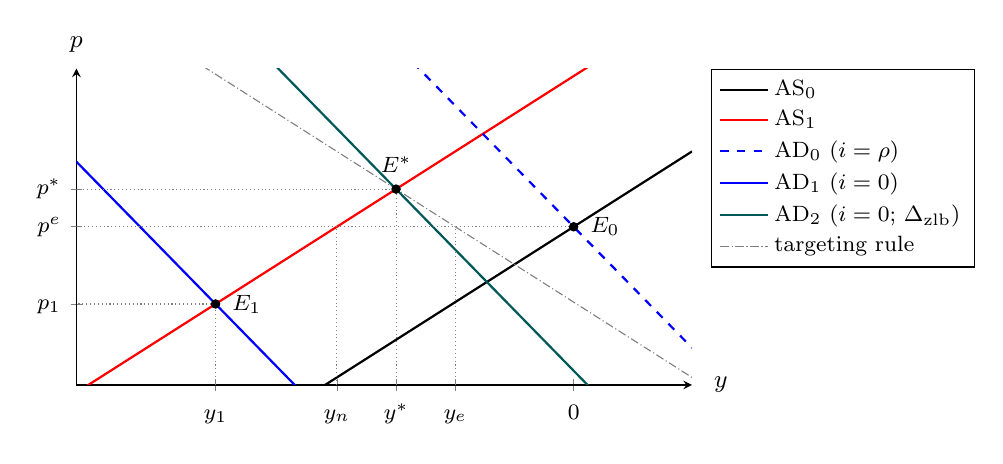
\begin{tikzpicture}
% admissible values, only to shape the curves: sigma=eta=1, alpha=.75, theta=1.5, chi=.6, d0=1, beta=.9; a=-.5, mu=1, abar=-1, dhat=-1.5
\pgfmathsetmacro{\Gsig}{1}\pgfmathsetmacro{\Geta}{1}\pgfmathsetmacro{\Galp}{0.75}\pgfmathsetmacro{\Gth}{1.5}
\pgfmathsetmacro{\Gchi}{0.6}\pgfmathsetmacro{\Gdz}{1}\pgfmathsetmacro{\Gbe}{0.9}\pgfmathsetmacro{\Grho}{-ln(\Gbe)}
\pgfmathsetmacro{\Ga}{-0.5}\pgfmathsetmacro{\Gmu}{1}\pgfmathsetmacro{\Gab}{-1}\pgfmathsetmacro{\Gdh}{-1.5}
\pgfmathsetmacro{\Gk}{(1-\Galp)*(1/\Gsig+\Geta)/\Galp}
\pgfmathsetmacro{\Gvp}{\Gsig-\Gdz*(1-\Gbe)*(1-\Gchi)/\Gchi}
\pgfmathsetmacro{\Gphi}{(\Gsig*\Gchi+(1-\Gchi)*\Gdz*\Gbe)/\Gchi}
\pgfmathsetmacro{\Gyn}{((1+\Geta)*\Ga-\Gmu)/(1/\Gsig+\Geta)}
\pgfmathsetmacro{\Gye}{(1+\Geta)*\Ga/(1/\Gsig+\Geta)}
\pgfmathsetmacro{\Gybn}{(1+\Geta)*\Gab/(1/\Gsig+\Geta)}
\pgfmathsetmacro{\Gin}{\Grho+(\Gybn-\Gyn+(1-\Gchi)/\Gchi*\Gdh)/\Gphi}
\pgfmathsetmacro{\Gm}{\Gmu/((1/\Gsig+\Geta)*(1+\Gth*\Gk))}
\pgfmathsetmacro{\Gzo}{\Gyn+\Gphi*\Gin}% zeta at i=0 after the shocks
\pgfmathsetmacro{\Gzs}{\Gyn+(1+\Gvp*\Gk)*\Gm}% zeta implementing y*
\pgfmathsetmacro{\Gyo}{\Gyn+\Gphi*\Gin/(1+\Gvp*\Gk)}\pgfmathsetmacro{\Gpo}{\Gk*(\Gyo-\Gyn)}
\pgfmathsetmacro{\Gys}{\Gyn+\Gm}\pgfmathsetmacro{\Gps}{\Gk*\Gm}
\begin{axis}[width=9.4cm,height=5.6cm,typeset ticklabels with strut,
  every axis x label/.style={at={(ticklabel* cs:1.02)},anchor=west},every axis y label/.style={at={(ticklabel* cs:1.02)},anchor=south},xmin=-2.1,xmax=0.5,ymin=-0.7,ymax=0.7,domain=-2.1:0.5,samples=2,axis lines=left,
  xtick={\Gyo,\Gyn,\Gys,\Gye,0},xticklabels={$y_1$,$y_n$,$y^*$,$y_e$,$0$},ytick={\Gpo,0,\Gps},yticklabels={$p_1$,$p^e$,$p^*$},
  xlabel={$y$},ylabel={$p$},tick label style={font=\footnotesize},label style={font=\small},
  legend style={font=\footnotesize},legend cell align=left,legend pos=outer north east]
\addplot[thick,black]{\Gk*x};
\addplot[thick,red]{\Gk*(x-\Gyn)};
\addplot[thick,blue,dashed]{-x/\Gvp};
\addplot[thick,blue]{(\Gzo-x)/\Gvp};
\addplot[thick,teal!70!black]{(\Gzs-x)/\Gvp};
\addplot[gray,densely dashdotted]{-(x-\Gye)/\Gth};
\legend{AS$_0$,AS$_1$,AD$_0$ ($i=\rho$),AD$_1$ ($i=0$),AD$_2$ ($i=0$; $\Delta_{\rm zlb}$),targeting rule}
\draw[gray,densely dotted] (axis cs:\Gyo,-0.7)--(axis cs:\Gyo,\Gpo)--(axis cs:-2.1,\Gpo);
\draw[gray,densely dotted] (axis cs:\Gys,-0.7)--(axis cs:\Gys,\Gps)--(axis cs:-2.1,\Gps);
\draw[gray,densely dotted] (axis cs:\Gyn,-0.7)--(axis cs:\Gyn,0) (axis cs:\Gye,-0.7)--(axis cs:\Gye,0) (axis cs:-2.1,0)--(axis cs:0,0);
\addplot[only marks,mark=*,mark size=1.5pt] coordinates {(0,0) (\Gyo,\Gpo) (\Gys,\Gps)};
\node[font=\footnotesize,anchor=west] at (axis cs:0.03,0) {$E_0$};
\node[font=\footnotesize,anchor=west] at (axis cs:\Gyo+0.03,\Gpo) {$E_1$};
\node[font=\footnotesize,anchor=south] at (axis cs:\Gys,\Gps+0.03) {$E^*$};
\end{axis}
\end{tikzpicture}
\end{center}
\intuicao{Rate and transfer both move the AD intercept, so for $(y,p)$ they are one instrument, and the transfer supplies what
the bound withholds. If transfers cost anything outside the loss (public debt, later distortionary taxes), cut the rate
first. As the optimum accommodates the markup shock, the bound binds for it before it binds for price stability.}
\refbib{Benigno (2015), \S9; \S11, eqs.\ (33)--(34); Romer (2012), \S11.6.}
\rubrica{
\item $y^*$, the implementing line and $i^*<i_n$: 1 pt.
\item The three options, $\Delta_{\rm zlb}$ and the welfare cost derived: 1 pt. Answered in the one-type model, without the borrowers' channel: max.\ half of (d).
\item Graph (1 pt; four lines of 0.25 pt): axes and symbolic labels; AS$_1$ through $(y_n,p^e)$; parallel AD shifts, AD$_2$ through $E^*$; $E_1$ below $p^e$, $E^*$ on AS$_1$ and the rule.
}
\end{sol}

\textbf{e)} (3 points) \emph{Parameter analysis.} Sign, with proofs, the effects of $\chi$, $d_0$ and $\kappa$ (through $\alpha$) on the transfer multiplier
and on $\Delta_{\rm zlb}$, and collect them in a table; compare with the multiplier when inflation between the short and the long run is constant instead; give the limits
and the stability conditions in both regimes; and read the results for Brazil's 2020 emergency transfers.
\resolespaco
\begin{sol}
\passo{multiplier --- part (c)}{$\chi(1+\varpi\kappa)=\chi(1+\sigma\kappa)-\kappa d_0(1-\beta)(1-\chi)$, so $\frac{\partial m_T}{\partial\chi}=-m_T^2[1+\sigma\kappa+\kappa d_0(1-\beta)]<0$,
$\frac{\partial m_T}{\partial d_0}=m_T^2\kappa(1-\beta)(1-\chi)>0$ and $\frac{\partial m_T}{\partial\kappa}=-m_T^2\chi\varpi$, negative iff $\varpi>0$.}
\passo{needed transfer --- part (d)}{$F\equiv(1-\chi)\Delta_{\rm zlb}=\chi(1+\varpi\kappa)\delta-\chi\varphi i_n$, with $\chi\varphi i_n=\chi\varphi\rho+\chi(\bar y_n-y_n)+(1-\chi)\hat d$ and $\chi\varphi=\sigma\chi+(1-\chi)\beta d_0$;
$y_n,\bar y_n$ depend on none of $\chi,d_0,\alpha$; $\delta$ on neither $\chi$ nor $d_0$ (it moves with $\alpha$ through $\kappa$). Hence
$\frac{\partial\Delta_{\rm zlb}}{\partial d_0}=-[\kappa(1-\beta)\delta+\beta\rho]<0$ and, as $(1+\varpi\kappa)\delta\propto\frac{1+\varpi\kappa}{1+\theta\kappa}$,
$\frac{\partial\Delta_{\rm zlb}}{\partial\kappa}=\frac{\chi}{1-\chi}\cdot\frac{\mu(\varpi-\theta)}{(\sigma^{-1}+\eta)(1+\theta\kappa)^2}$. $F$ is affine in $\chi$, so $\frac{\partial\Delta_{\rm zlb}}{\partial\chi}=\frac{F'(1-\chi)+F}{(1-\chi)^2}=\frac{F(1)}{(1-\chi)^2}$, with
$F(1)=(1+\sigma\kappa)\delta-\sigma\rho-(\bar y_n-y_n)=-\sigma i^*_{\rm RA}$, where $i^*_{\rm RA}$ is $i^*$ at $\chi=1$: the optimal rate of a one-type economy.}
\passo{constant inflation --- $\bar p_n-p$ fixed in (32)}{Only the Fisher term moves with $p$: $dy=\frac{1-\chi}\chi\Delta+\frac{(1-\chi)d_0}\chi\kappa\,dy$, so $m_T^c=\frac{1}{\chi-(1-\chi)d_0\kappa}$,
with $\frac{\partial m_T^c}{\partial\chi}=-(m_T^c)^2(1+d_0\kappa)<0$, $\frac{\partial m_T^c}{\partial d_0}=(m_T^c)^2(1-\chi)\kappa>0$, $\frac{\partial m_T^c}{\partial\kappa}=(m_T^c)^2(1-\chi)d_0>0$; and $\frac1{m_T}-\frac1{m_T^c}=\kappa\chi\varphi>0$, so
$m_T^c>m_T$.}
\begin{center}\small
\begin{tabular}{lccc}
\toprule
 & $\chi$ & $d_0$ & $\kappa$ (through $\alpha$)\\
\midrule
$m_T=1/[\chi(1+\varpi\kappa)]$, anchored long run & $-$ & $+$ & $-$ iff $\varpi>0$\\
$m_T^c=1/[\chi-(1-\chi)d_0\kappa]$, constant inflation & $-$ & $+$ & $+$\\
$\Delta_{\rm zlb}$, transfer per borrower at $i=0$ & $+$ iff $i^*_{\rm RA}<0$ & $-$ & $-$ iff $\varpi<\theta$\\
\bottomrule
\end{tabular}
\end{center}
\passo{limits and stability}{$\kappa\to0$: $m_T,m_T^c\to\frac1\chi$ (the fixed-price cross). $\kappa\to\infty$ with $\varpi>0$: $m_T\to0$ (output stays at $y_n$). $d_0\to0$: $m_T\to\frac1{\chi(1+\sigma\kappa)}$,
$m_T^c\to\frac1\chi$. $\chi\to1$: $m_T\to\frac1{1+\sigma\kappa}$, $m_T^c\to1$, and $\Delta_{\rm zlb}\to+\infty$ if $i^*_{\rm RA}<0$. Stability (footnote 19: the AS flatter than an upward-sloping AD):
anchored, $\kappa<-1/\varpi$ when $\varpi<0$, i.e.\ $1+\varpi\kappa>0$, automatic when $\varpi>0$; constant inflation, $\kappa<\frac{\chi}{(1-\chi)d_0}$, i.e.\ $m_T^c>0$. At each knife
edge the multiplier diverges ($1+\varpi\kappa\to0^+$, $\kappa\to\chi/[(1-\chi)d_0]^-$).}
\passo{reading}{$m_T$ falls with $\chi$ (fewer households re-spend income, and the real-rate brake $\varpi$ rises toward $\sigma$), rises with $d_0$
(the inflation a transfer creates erodes more debt), and falls with $\kappa$ when $\varpi>0$ (flexible prices turn the push into inflation,
which raises the real rate); under constant inflation the $\kappa$ sign flips and the slump from $\hat d$, $m_T^c(1-\chi)\hat d$, deepens with $\kappa$
(paradox of flexibility). $\Delta_{\rm zlb}$ falls with $d_0$ (the cut to zero eases the borrowing limit more and $m_T$ is larger) and with $\kappa$ unless $\varpi>\theta$
(the rule accommodates less of the markup shock); it rises with $\chi$ when a one-type economy would itself need $i^*<0$.}
\passo{Brazil, 2020}{The \emph{aux\'{\i}lio emergencial} paid lump sums to informal and low-income households, the closest analogue of $\Delta$
(households at their limit spend a transfer one for one). (1) Targeting sets the effect: a transfer spread over all households
reaches borrowers only in proportion $1-\chi$; the part paid to savers does nothing. (2) Debt raises $m_T$ and lowers the transfer
needed while long-run prices stay anchored; if inflation expectations de-anchor, $m_T^c>m_T$ but stability needs $\kappa<\chi/[(1-\chi)d_0]$. (3) The Selic stayed above zero, but an effective lower bound $\underline i>0$ (risk
premia, fiscal risk) works the same way: replace $-i^*$ by $\underline i-i^*$ in $\Delta_{\rm zlb}$. (4) After a cost-push shock the optimum has $p^*>p^e$:
some inflation belongs to the optimal mix, and only a transfer above $\Delta_{\rm zlb}$ moves the economy up AS$_1$ past $E^*$.}
\intuicao{Every sign weighs how much of a demand push survives the price response against how much of the economy
re-spends income; anchoring of the long run decides whether price flexibility helps or hurts.}
\refbib{Benigno (2015), \S10, footnotes 19--20 and the multipliers on p.~521; \S11; Romer (2012), \S8.6, \S11.6, \S12.2.}
\rubrica{
\item Signs of $m_T$ and $m_T^c$ with their derivatives: 1 pt. Signs listed without derivatives: 0 for those lines.
\item Signs of $\Delta_{\rm zlb}$, including the affine argument for $\chi$: 0.75 pt.
\item Limits and both stability conditions: 0.5 pt.
\item Reading, including Brazil: 0.75 pt. Table without proofs or without reading: max.\ half of (e).
}
\end{sol}
